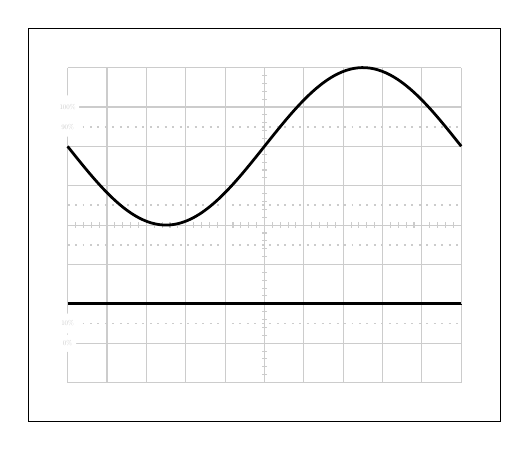
\begin{tikzpicture}[scale=0.5,every node/.style={transform shape}]
\def\angC{180}
    %Lineas intermedias grilla
    \foreach \x in {-5,-4.8,...,4.8,5}{
        \draw[gray!40,thin,shift={(\x,0)}] (0pt,2pt) -- (0pt,-2pt);
    }
    \foreach \y in {-4,-3.8,...,3.8,4}{
        \draw[gray!40,thin,shift={(0,\y)}] (2pt,0pt) -- (-2pt,0pt);
    }
    \foreach \a [evaluate={\y=\a*0.5}] in {-5,-1,1,5}{
        \draw[gray!40,line width=0.7pt,dotted] (-5,\y) -- (5,\y);
    }

    %Grilla
    \draw[thin,gray!40] (-5,-4) grid (5,4);
    \node[fill=white,text=gray!40,circle,scale=0.5] at (-5,3) {$100\%$};
    \node[fill=white,text=gray!40,circle,scale=0.5] at (-5,2.5) {$90\%$};
    \node[fill=white,text=gray!40,circle,scale=0.5] at (-5,-2.5) {$10\%$};
    \node[fill=white,text=gray!40,circle,scale=0.5] at (-5,-3) {$0\%$};
    \draw[black] (-6,-5) rectangle(6,5);
    
    
    \draw [line width=1pt,black] plot[smooth,samples=100,domain=-5:5](\x,{2*sin(deg(\x*pi*0.2))+2});

    
    \draw [thin,black] plot[smooth,samples=100,domain=\angC/36:5](\x,{2*sin(deg(\x*pi*0.2))-2});
    \draw [thin,black] plot[smooth,samples=100,domain=-5+\angC/36:0](\x,{2*sin(deg(\x*pi*0.2))-2});
    \draw[thin,black](\angC/36,{2*sin(deg(3.14*\angC/36*0.2))-2})--(\angC/36,-2);
    \draw[thin,black](-5+\angC/36,{2*sin(deg(3.14*(-5+\angC/36)*0.2))-2})--(-5+\angC/36,-2);
    \draw[line width=1pt,black](-5,-2)--(-5+\angC/36,-2) (0,-2)--(\angC/36,-2);
\end{tikzpicture}
\caption*{$Ang_{cond}=0$}